\documentclass[notheorems,mathserif,table,compress]{beamer}  %dvipdfm选项是关键,否则编译统统通不过
%%------------------------常用宏包------------------------
%%注意, beamer 会默认使用下列宏包: amsthm, graphicx, hyperref, color, xcolor, 等等
\usepackage{fontspec,xunicode,xltxtra}  % for XeTeX
\usepackage{graphicx}
\usepackage{fancybox}
\usepackage{comment}
\usepackage{booktabs}
\usepackage{colortbl}
\usepackage{tcolorbox}
\usepackage{pifont}
%%------------------------ThemeColorFont------------------------
%% Presentation Themes
% \usetheme[<options>]{<name list>}
\usetheme{Madrid}
%% Inner Themes
% \useinnertheme[<options>]{<name>}
%% Outer Themes
% \useoutertheme[<options>]{<name>}
\useoutertheme{miniframes} 
%% Color Themes 
% \usecolortheme[<options>]{<name list>}
%% Font Themes
% \usefonttheme[<options>]{<name>}
\setbeamertemplate{background canvas}[vertical shading][bottom=white,top=structure.fg!7] %%背景色, 上25%的蓝, 过渡到下白.
\setbeamertemplate{theorems}[numbered]
\setbeamertemplate{navigation symbols}{}   %% 去掉页面下方默认的导航条.

\usepackage{zhfontcfg}
\usepackage{subfigure}
\usepackage{pgf}
\usepackage{color}
\usepackage{caption}

%\setsansfont[Mapping=tex-text]{文泉驿正黑}  %% 需要fontspec宏包
     %如果装了Adobe Acrobat,可在font.conf中配置Adobe字体的路径以使用其中文字体
     %也可直接使用系统中的中文字体如SimSun,SimHei,微软雅黑 等
     %原来beamer用的字体是sans family;注意Mapping的大小写,不能写错
     %设置字体时也可以直接用字体名,以下三种方式等同:
     %\setromanfont[BoldFont={黑体}]{宋体}
     %\setromanfont[BoldFont={SimHei}]{SimSun}
     %\setromanfont[BoldFont={"[simhei.ttf]"}]{"[simsun.ttc]"}
%%------------------------MISC------------------------
\graphicspath{{figures/}}         %% 图片路径. 本文的图片都放在这个文件夹里了.
%%------------------------正文------------------------
%\pgfputat{\pgfxy(3,-6)}{\pgfbox[centering,base]{
\includegraphics[width=2cm,height=2cm]{figures/ouc}}}
\begin{document}

\XeTeXlinebreaklocale "zh"         % 表示用中文的断行
\XeTeXlinebreakskip = 0pt plus 1pt % 多一点调整的空间
%%----------------------------------------------------------
%% This is only inserted into the PDF information catalog. Can be left
%% out.
%%%
%% Delete this, if you do not want the table of contents to pop up at
%% the beginning of each subsection:
\AtBeginSection[]{                              % 在每个Section前都会加入的Frame
  \frame<handout:0>{
    \frametitle{下一节内容}\small
    \tableofcontents[current,currentsubsection]
  }
}
\AtBeginSubsection[]                            % 在每个子段落之前
{
  \frame<handout:0>                             % handout:0 表示只在手稿中出现
  {
    \frametitle{下一节内容}\small
    \tableofcontents[current,currentsubsection] % 显示在目录中加亮的当前章节
  }
}
%%----------------------------------------------------------
\title{基于环结构特征的视网膜血管图像配准}

 \author[邱欣欣]{\hspace{-2em}答辩人~~\textcolor{olive}{邱~欣~欣}\\
                             \hspace{-1em}导师~~\textcolor{olive}{郑~海~永}\\
                             \hspace{-1.7em}\hspace{4em}专业~~\textcolor{olive}{信号与信息处理}}
    \institute[中国海洋大学]{\small \kai \textcolor{violet}{中国海洋大学\\信息科学与工程学院}}
\date{2016~年~5~月~22~日}
\titlegraphic{

\includegraphics[height=2cm]{ouc}}
%\begin{figure}
%\centering
%    
\includegraphics[width=4cm]{figures/ouc}\medskip
%\end{figure}
%\titlegraphic{\vspace{-6em}
\includegraphics[height=7cm]{ouc}\vspace{-6em}}
\frame{ \titlepage }
%%----------------------------------------------------------
%\section*{Content}
\frame{\frametitle{内容提要}\tableofcontents}
%%----------------------------------------------------------
\small
\newcommand{\shadow}[2][blue]{\hskip5pt\shadowbox{\color{#1}\small #2\vspace{3mm}}}
\newcommand{\shado}[2][blue]{\hskip5pt\shadowbox{\color{#1}\Huge #2\vspace{3mm}}}
\setbeamertemplate{caption}{\raggedright\insertcaption\par}
\section{课题背景}


\begin{frame}
\frametitle{视网膜图像配准}
 \shadow{图像配准}将不同时间、不同传感器(成像设备)或不同条件下(天候、照度、摄像位置和角度等)获取的两幅或多幅图像进行匹配、叠加的过程。
 \begin{figure}[ht!]
    \centering
  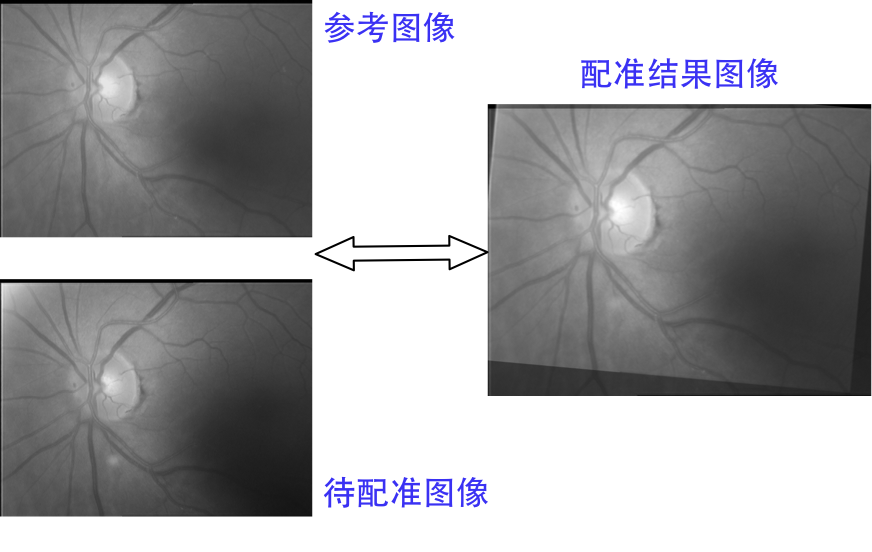
\includegraphics[width=0.6\linewidth]{配准示例.png}
 \end{figure}
视网膜图像配准在医学上对于眼科医师进行眼科疾病的预防、诊断与治疗具有重要意义。
\end{frame}


\begin{frame}
\frametitle{国内外研究现状}
目前广泛使用的主要有两类图像配准方法:
\begin{itemize}
\item {\color{blue}{基于灰度信息的配准方法}} %复杂度较高,对图像质量要求较高
\item {\color{blue}{基于特征的配准方法}} %计算量较低、对图像灰度变化有一定的鲁棒性,但对特征提取、 特征匹配的准确性要求较高
\end{itemize}
视网膜图像拥有较鲁棒的特征如血管网络、视神经盘等,因此基于特征的方法对视网膜图像配准来说更为有效。常用的基于特征的视网膜配准方法有:
\begin{itemize}
\item 点特征配准算法:分级的基于 landmark 特征的方法、Dual-Bootstrap 迭代最近点算法、Generalized Dual-Bootstrap 迭代最近点算法等
\begin{itemize}
\item {\color{red}{依赖于单个分叉点或交叉点的分支角度,易造成错配}}
\end{itemize}
\item 结构特征配准算法:Bifurcation结构等 
\begin{itemize}
\item {\color{red}{准确性提高,但对分割结果要求较高,对血管细节较敏感}}
\end{itemize}
\end{itemize}

\end{frame}

 \begin{frame}
\frametitle{算法基本流程}
基于多尺度和多环特征的从局部到全局的视网膜配准基本流程
 \begin{figure}[ht!]
    \centering
  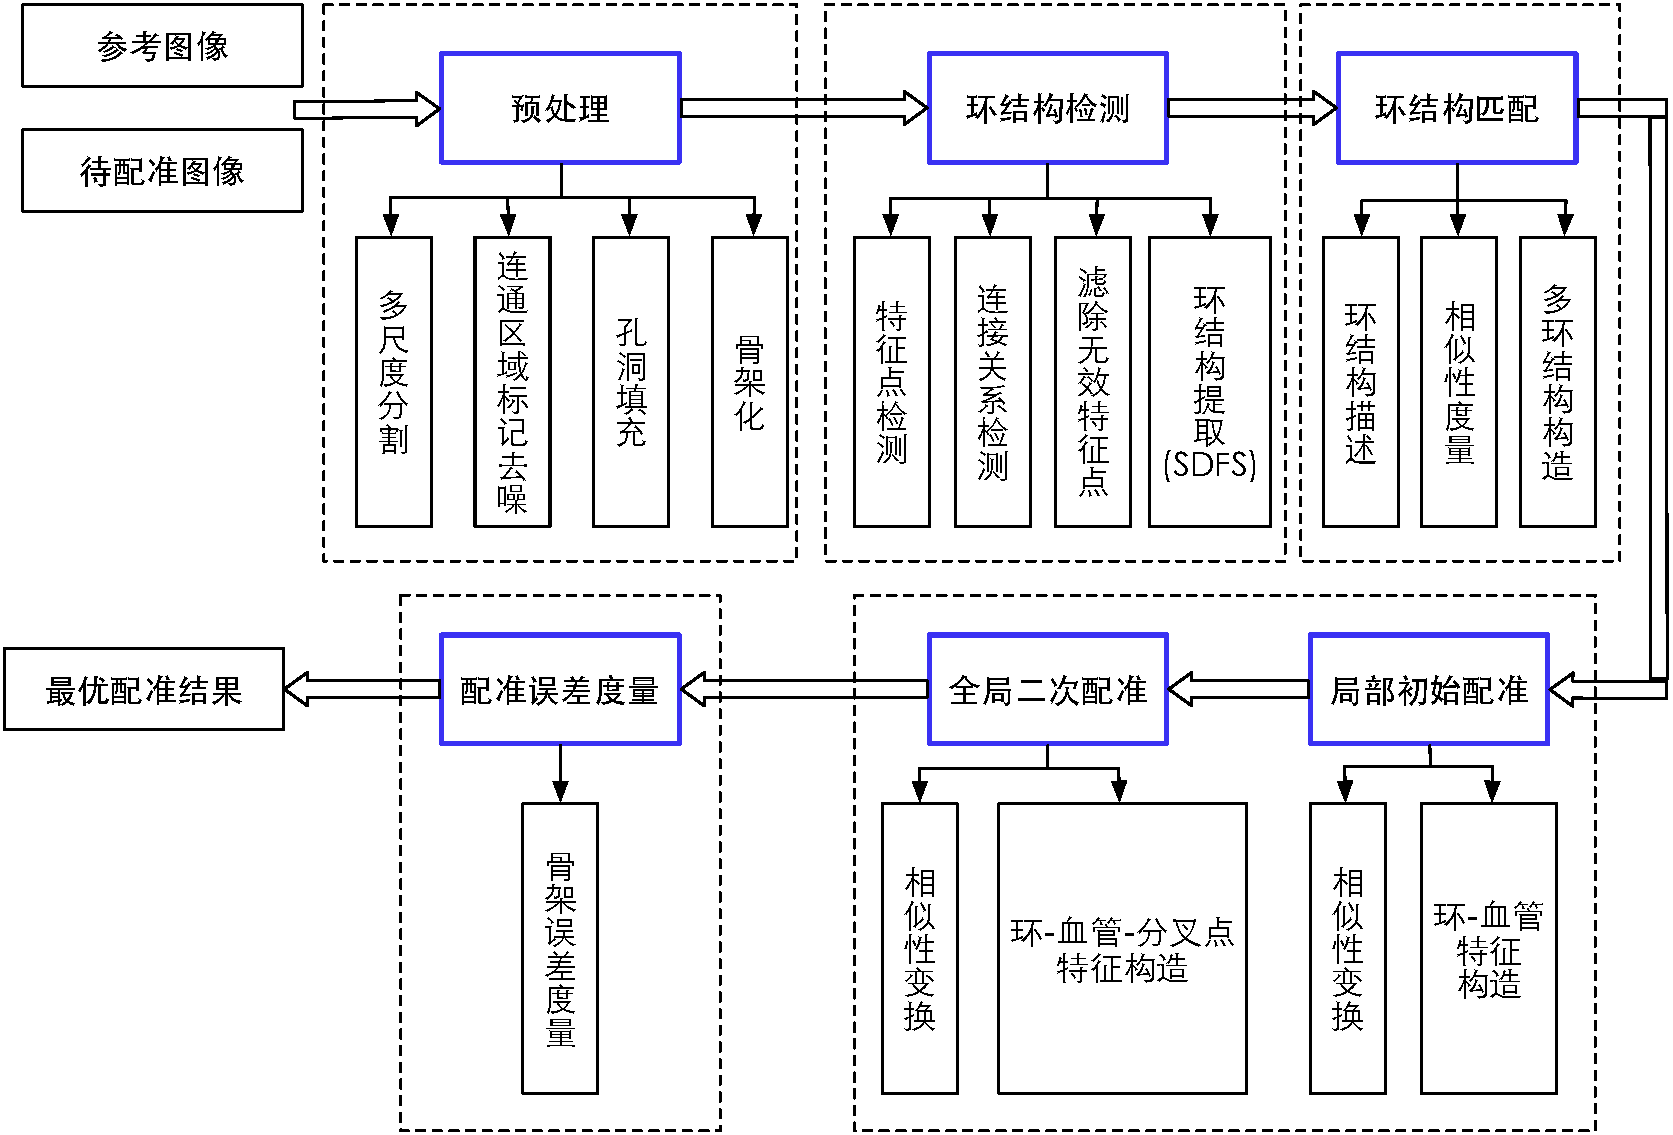
\includegraphics[width=0.8\linewidth]{流程图}
 \end{figure}
 \end{frame}
 
\section{研究内容}
\subsection{图像预处理}

 \begin{frame}
\frametitle{预处理步骤}
{\color{blue}{\ding{172}~多尺度分割}} 选择基于多尺度和多小波核的视网膜血管分割方法用来进行多尺度的血管分割\footnote{Wang Y, Ji G, Lin P, et al. Retinal vessel segmentation using multiwavelet kernels and multi- scale hierarchical decomposition. Pattern Recognition, 2013, 46(8):2117–2133.}。
\begin{itemize}
\item {\color{red}{不同尺度的分割结果代表不同程度的细节信息,我们选择其中的14个尺度。}}
\item {\color{red}{可有效避免因分割结果不理想造成的特征提取失败。}}
\end{itemize}
{\color{blue}{\ding{173}~连通区域标记去噪}} 采用8连通(上、下、左、右、左上角、左下角、右上角或右下角)进行标记。

{\color{blue}{\ding{174}~孔洞填充}} 膨胀、腐蚀。

{\color{blue}{\ding{175}~骨架化}} 轮廓修建骨架化方法\footnote{http://www.cs.smith.edu/∼nhowe/research/code/}。
 \end{frame}


\begin{frame}
\frametitle{预处理流程}
 \begin{figure}[ht!]
   \centering
  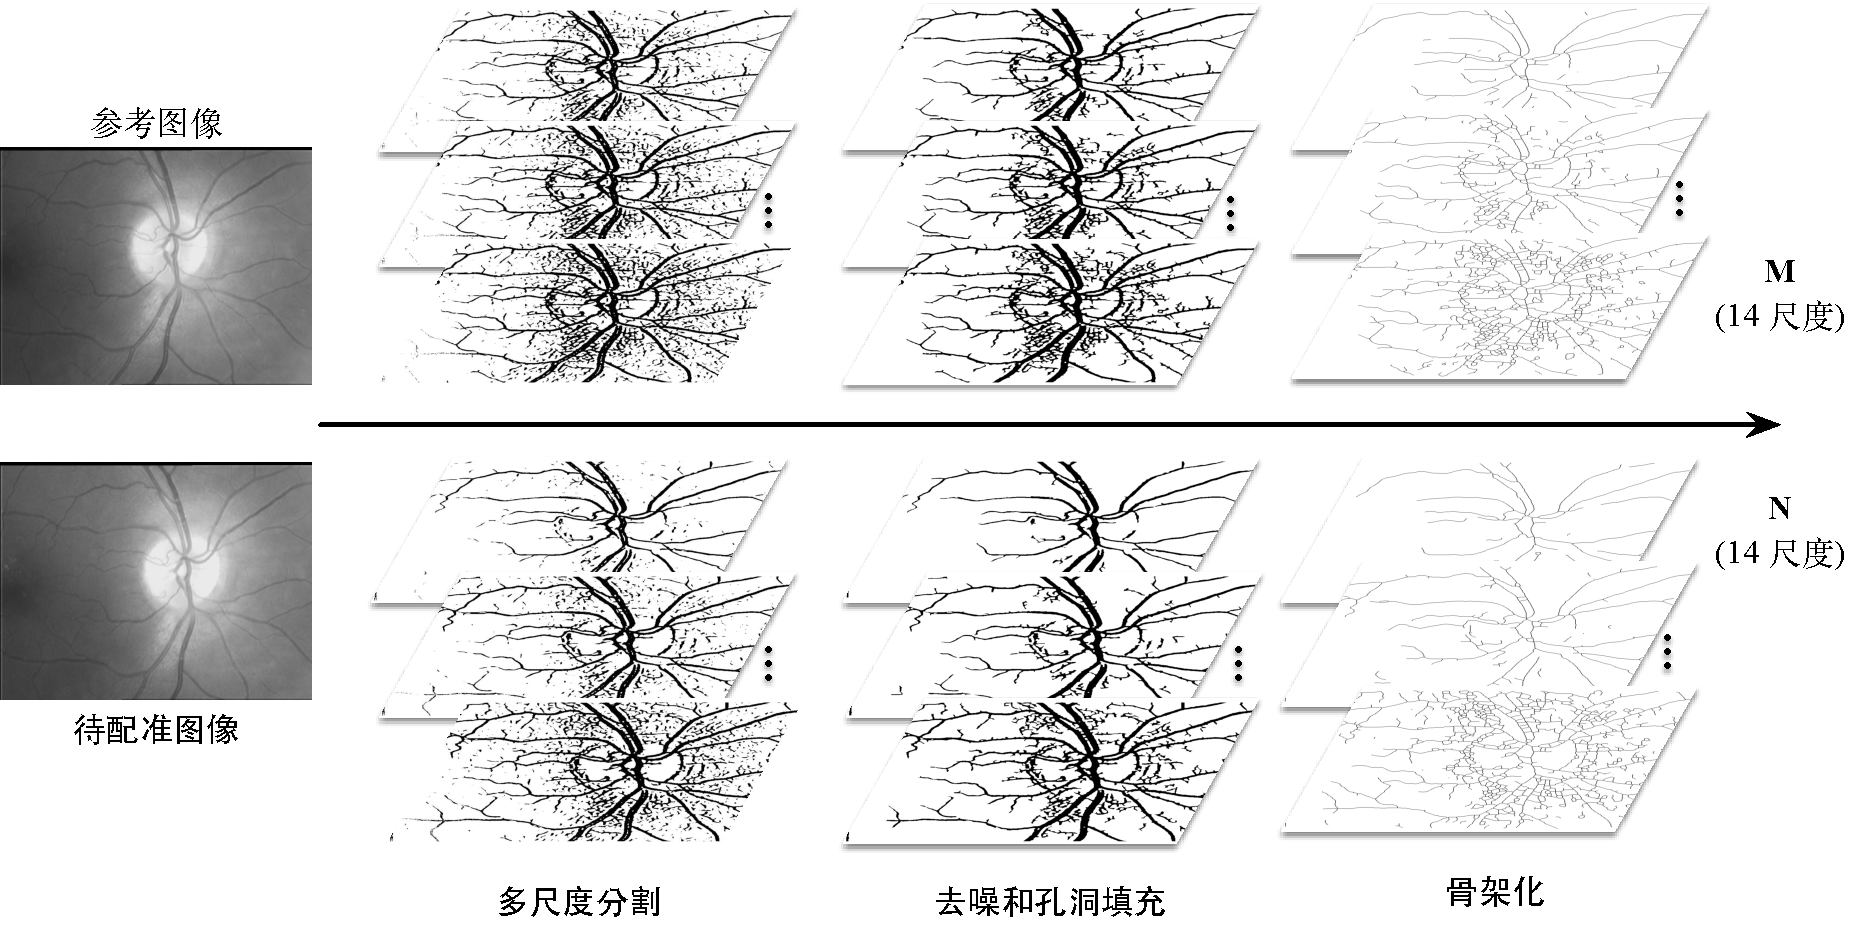
\includegraphics[width=\linewidth]{预处理}
  \caption{预处理流程}
 \end{figure}
\end{frame}

\subsection{环结构检测}

 \begin{frame}
 \frametitle{环结构概念}
 \shadow{环结构}由动脉和静脉的血管的分叉点、交叉点及相连接的血管组成的结构。
 
 具有较好的
  \begin{figure}[ht!]
    \centering
  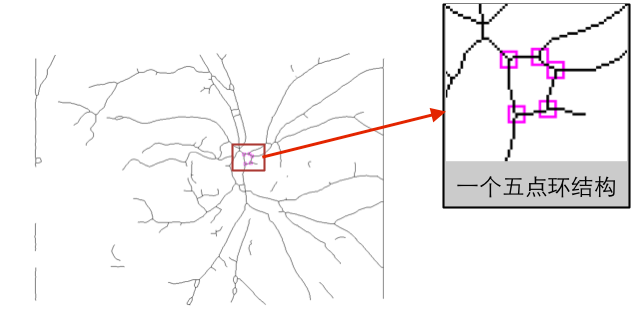
\includegraphics[width=0.75\linewidth]{五点环.png}
 \end{figure}
\setlength{\fboxsep}{2pt}%
\centering
\doublebox{%
\begin{minipage}{11cm}
由三个分叉点(或交叉点)组成的环结构称作三点环,依次类推。
\end{minipage}}
\end{frame}

 \begin{frame}
 \frametitle{环结构检测步骤}
{\color{blue}{\ding{172}~特征点(分叉点、交叉点)检测}}:一个像素其8邻域内像素值为 1 的个数大于等于 3,
       则这个像素有可能为分叉点(交叉点)。

{\color{blue}{\ding{173}~特征点连接关系检测}}:以一个特征点为起点,沿其八邻域逐渐向外搜索。

{\color{blue}{\ding{174}~无效特征点滤除}}:无效特征点即不能构成环的特征点,通过迭代去除度等于 1 的特征点。

{\color{blue}{\ding{175}~基于空间信息的深度优先搜索算法(SDFS)提取环结构。}}%$\Longrightarrow$
\begin{itemize}
\item 利用图像的坐标信息$+$深度优先搜索。
\item 输出所有组成环的特征点。
\end{itemize}
\end{frame}

\begin{frame}
 \frametitle{环结构检测步骤}
\setlength{\fboxsep}{2pt}%
     \doublebox{%
       \begin{minipage}{11cm}
SDFS算法可以求出所有点环,但在实验中只选择三、四、五点环来作为配准特征。
       \end{minipage}}
  \begin{figure}[ht!]
   \centering
  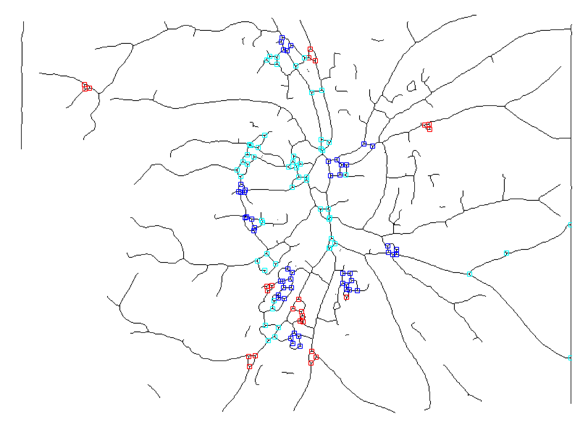
\includegraphics[width=0.4\linewidth]{345cycle.png}
  \caption{一幅视网膜图像的三、四、五点环结构图}
    \label{345cycle}
 \end{figure}
\end{frame}


\subsection{环结构匹配}

 \begin{frame}
 \frametitle{环结构描述和相似性度量}
 \begin{columns}
\column{.5\textwidth}
\begin{figure}[ht!]
\centering
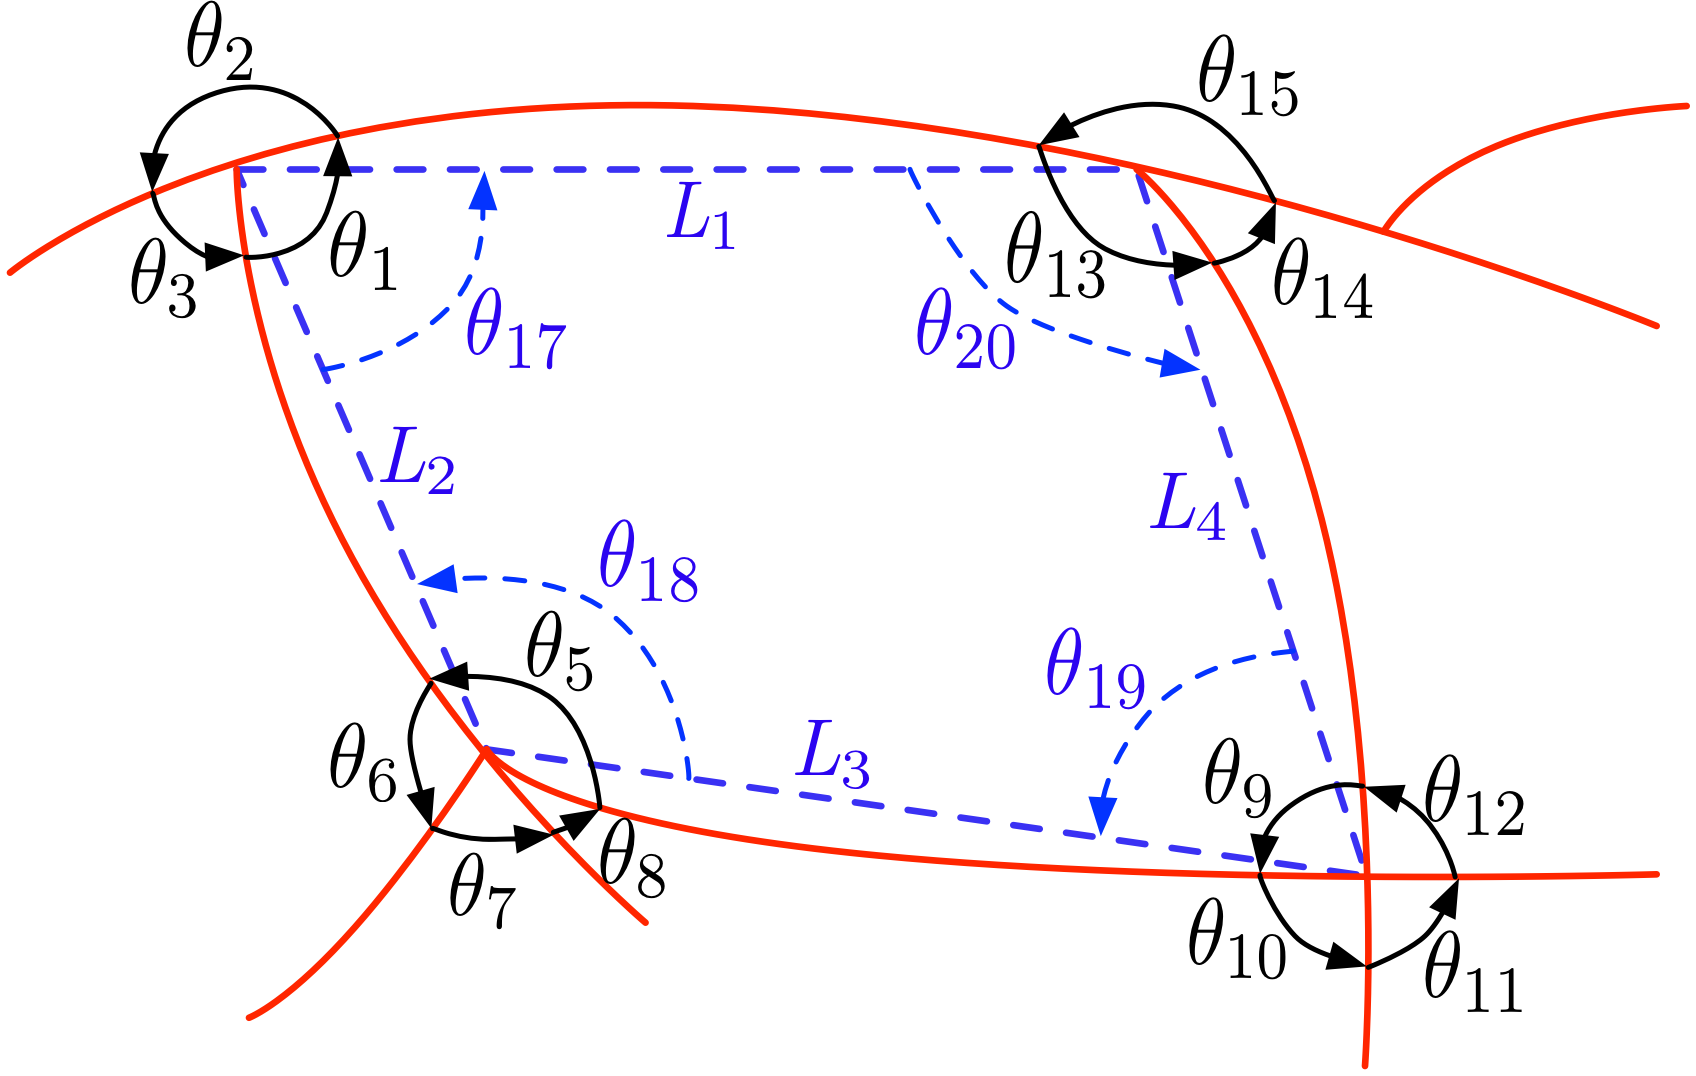
\includegraphics[width=0.8\linewidth]{description.png}
\caption{四点环实例}
 \end{figure}
  \begin{equation*}
 \begin{split}
\tilde{v}=\{L_{1},L_{2},L_{3},L_{4},\theta_{1},\theta_{2},\theta_{3},\mathbf{0},\theta_{5},\theta_{6},\theta_{7},\\\theta_{8},\theta_{9},\theta_{10},\theta_{11},\theta_{12},\theta_{13},\theta_{14},\theta_{15},\mathbf{0},\theta_{17},\\\theta_{18},\theta_{19},\theta_{20}\}
 \end{split}
 \end{equation*}
\column{.5\textwidth}
相似性度量完成参考图像与待配准图像中相同特征点数的环结构的匹配工作,采用的为{\color{blue}{曼哈顿距离}}:
 \begin{align*}
D_{pq} = mean(|V_p-W_q|),\\
 p = 1, 2, \ldots, m; q = 1, 2, \ldots, n
\end{align*}
$V_p$:参考图像图像中的第$P$个环结构的向量,$W_q$:待配准图像中的第$q$个环结构的向量,函数mean:向量求均值运算。
	
{\color{red}{$D_{pq}$的值越小,表明两个环结构相似性越高}} 	

所有三、四、五点环匹配对,只选择其中相似性度量值最小的一组。
\end{columns}
\end{frame}


\begin{frame}
\frametitle{环结构特征匹配结果}
   \begin{figure}[ht!]
    \centering
  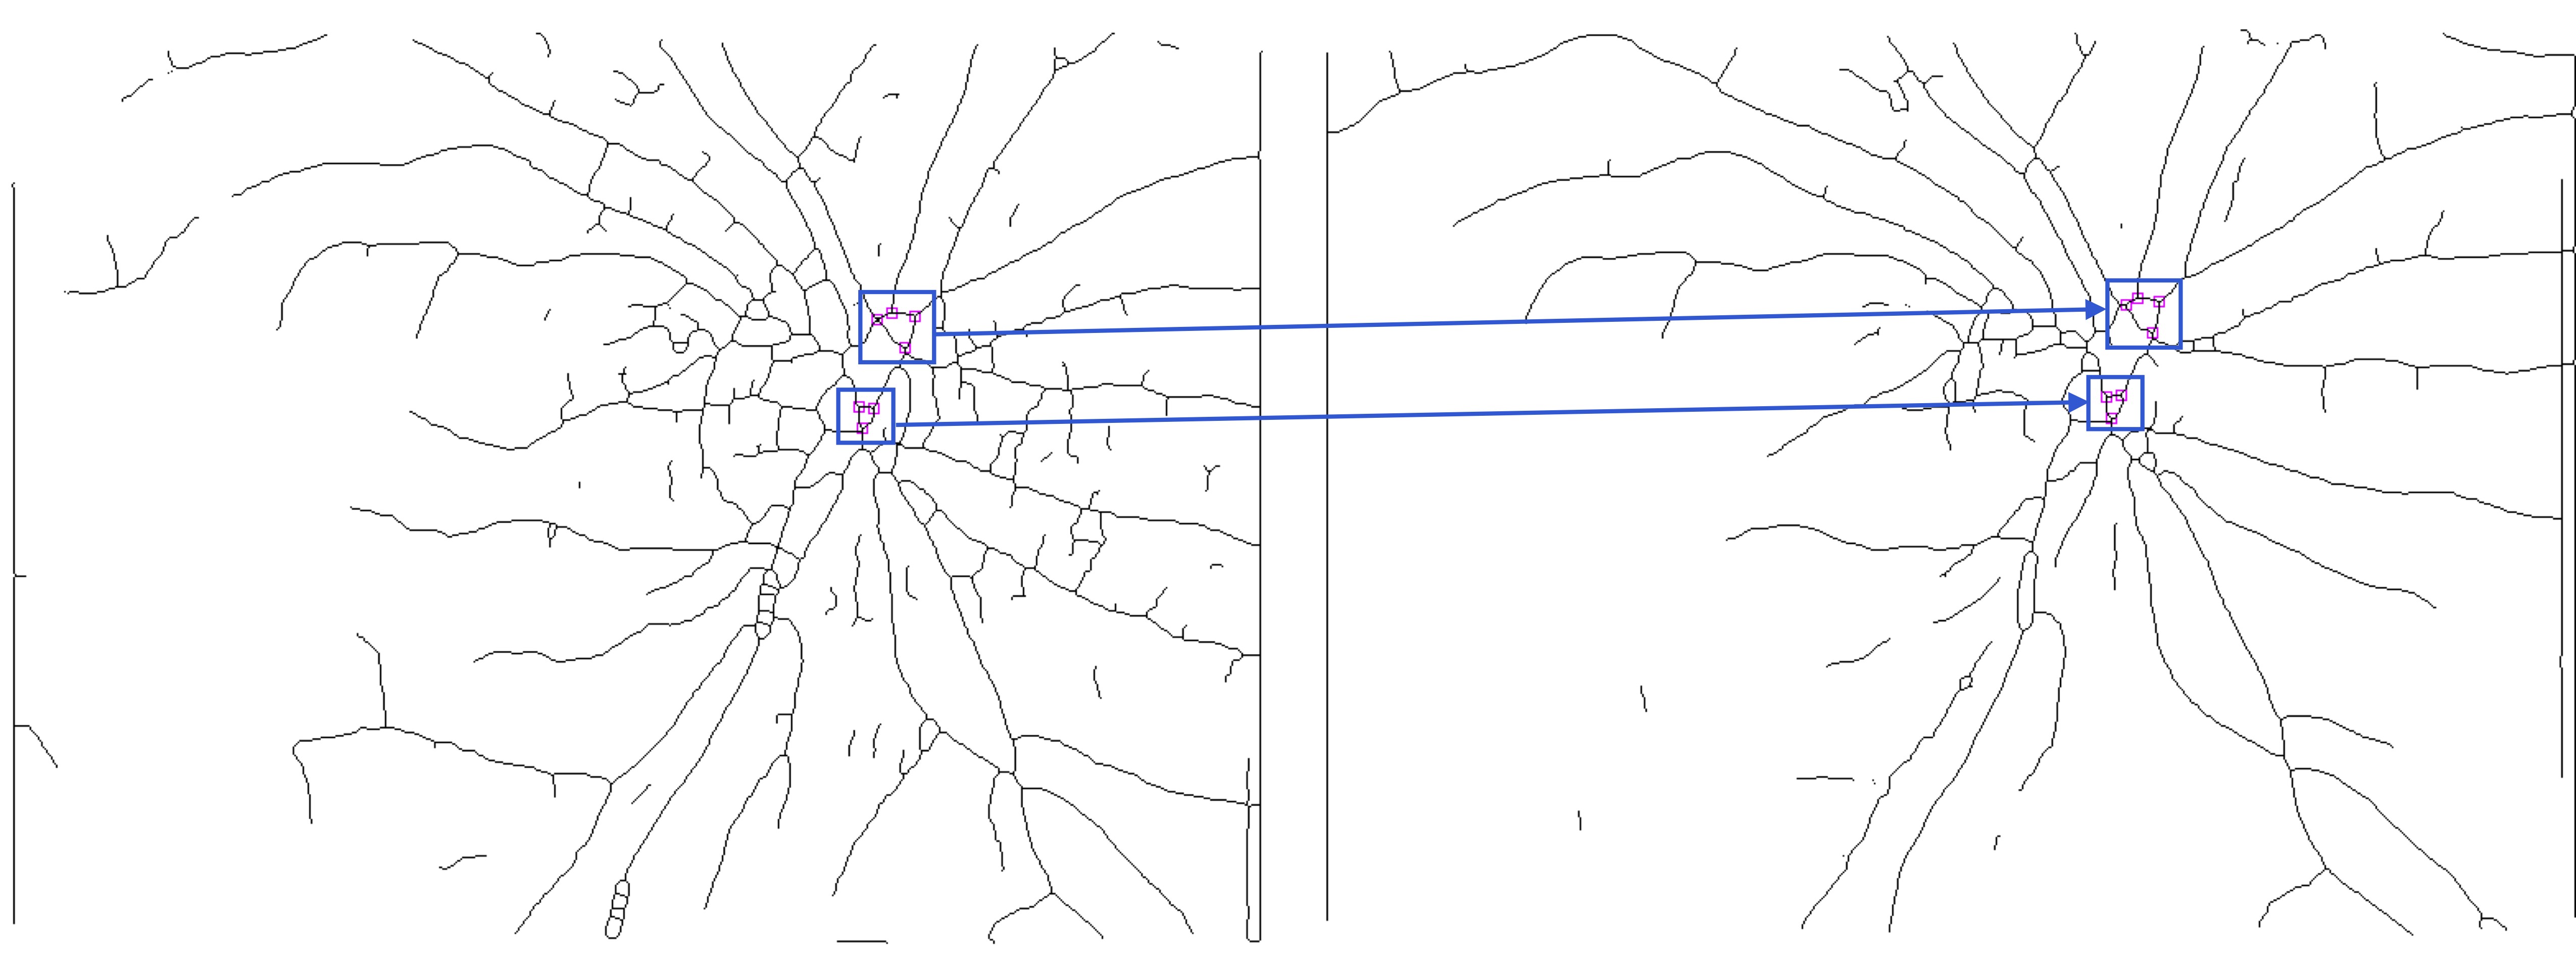
\includegraphics[width=\linewidth]{207-208}
  \caption{参考图像与待配准图像匹配的最优三、四点环}
 \end{figure}
\end{frame}

 \begin{frame}
 \frametitle{多环结构构造}
 不同类型的最优环结构组合在一起,可能会产生不同的配准结果,因此我们将三、四、五点环结构随机组合,得到多环结构。
    \begin{figure}[ht!]
    \centering
  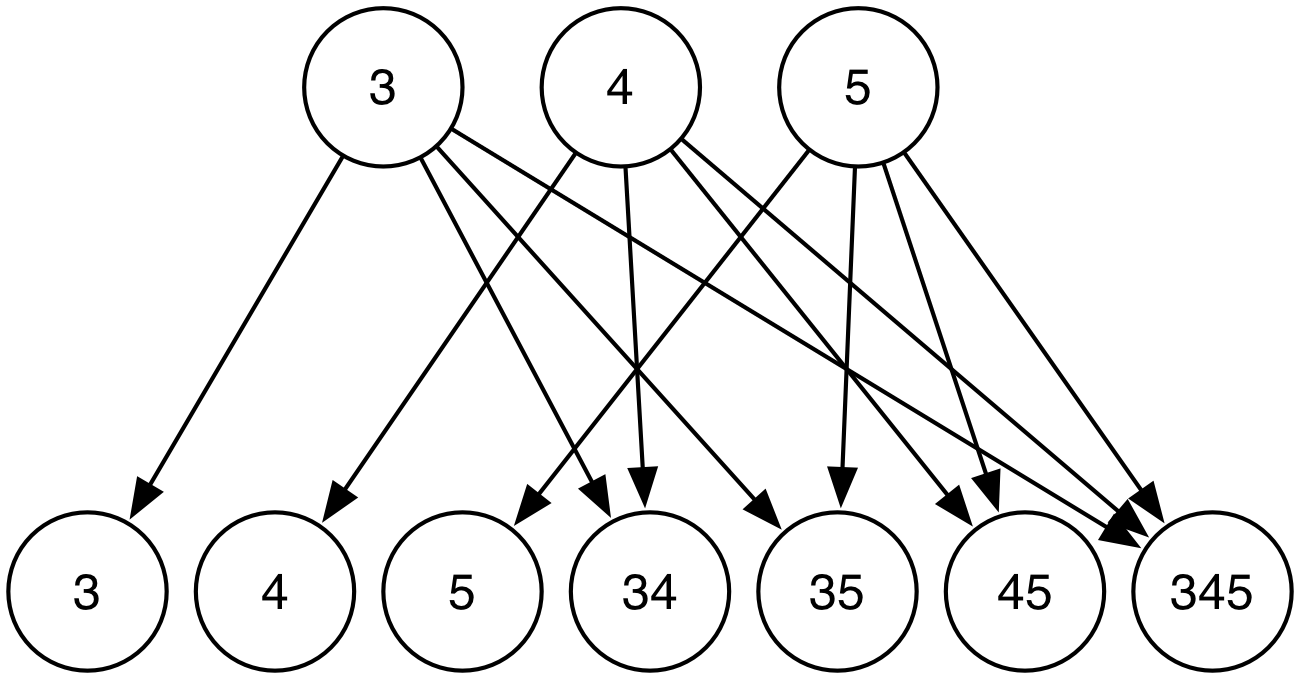
\includegraphics[width=0.6\linewidth]{345.png}
  \caption{多环组合}
 \end{figure}
 \setlength{\fboxsep}{2pt}%
\centering
\doublebox{%
\begin{minipage}{11cm}
同一尺度下,每对待配准图像最多会有7种环结构组合配准结果。
\end{minipage}}
\end{frame}

\subsection{从局部到全局的配准策略}

 \begin{frame}
 \frametitle{环-血管特征}
{\color{blue}{环结构}}:{\color{red}{缺点:有限特征点、视网膜血管信息未考虑到}}。
 
{\color{blue}{环-血管结构 }}:由环结构特征点,与其最近的分叉点、交叉点,及两者之间的血管中点组成。
    \begin{figure}[ht!]
    \centering
  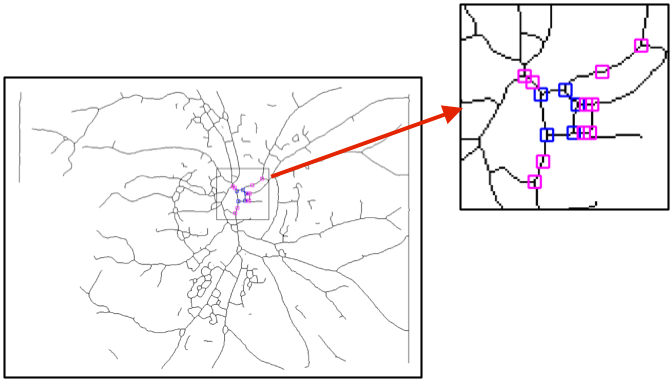
\includegraphics[width=0.7\linewidth]{环血管.png}
  \caption{环-血管结构}
 \end{figure}
\end{frame}

 \begin{frame}
 \frametitle{变换模型-相似性变换}
 常用的图像配准变换模型有{\color{blue}{相似性变换}}、{\color{blue}{仿射变换}}、{\color{blue}{多项式变换}}等。
 
 环 -血管结构对于平移、旋转和缩放是不变的,因此选择相似性变换作为配准的变换模型,其定义如下:
 \begin{equation}
\begin{split}		
X=xs\cos\phi-ys\sin\phi+a\\
Y=xs\sin\phi+ys\cos\phi+b	
\end{split}
\end{equation}
其中$s$代表尺度,$\phi$代表旋转角度,$(a,b)$代表了参考图像与待配准图像间的平移距离。
\end{frame}

 \begin{frame}
 \frametitle{局部初始配准}
 \begin{figure}[ht!]
 \setcounter{subfigure}{0}
  \subfigure[参考图像]{
  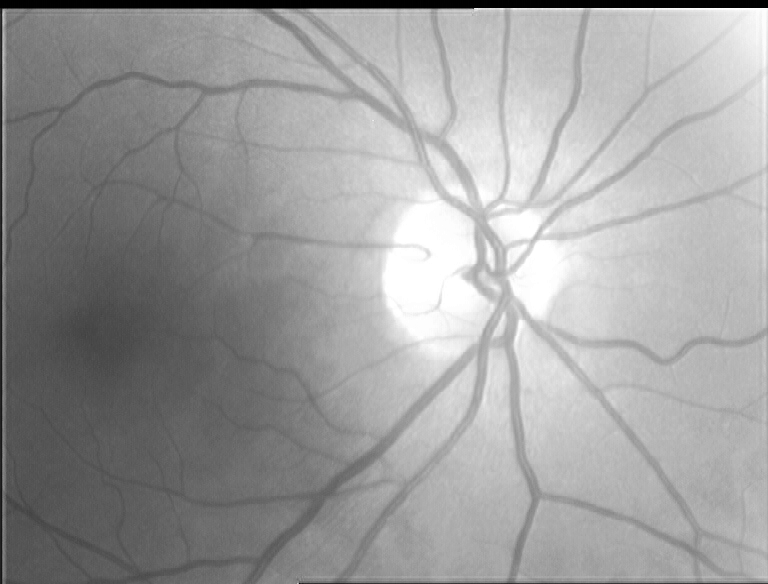
\includegraphics[width=0.3\linewidth]{R128.png}}
\hspace{0.1in}
\subfigure[待配准图像]{
  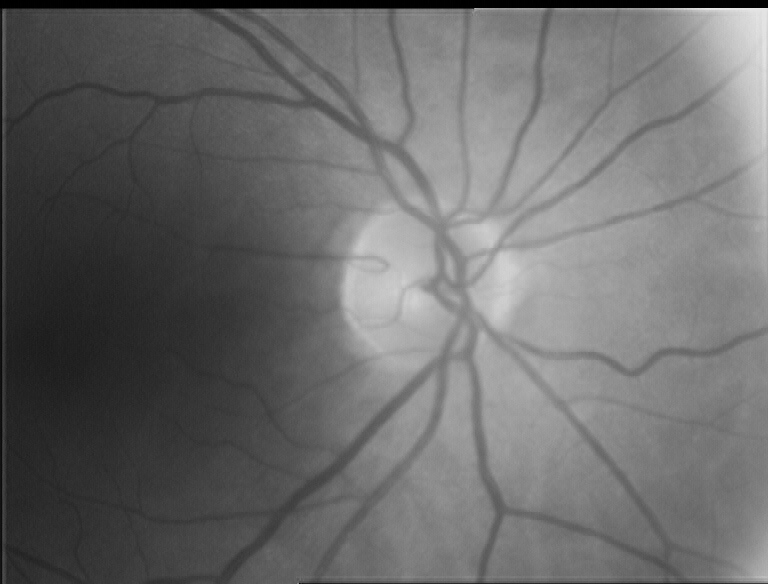
\includegraphics[width=0.3\linewidth]{R225.png}}
  \\
    \subfigure[骨架化图像配准结果]{
  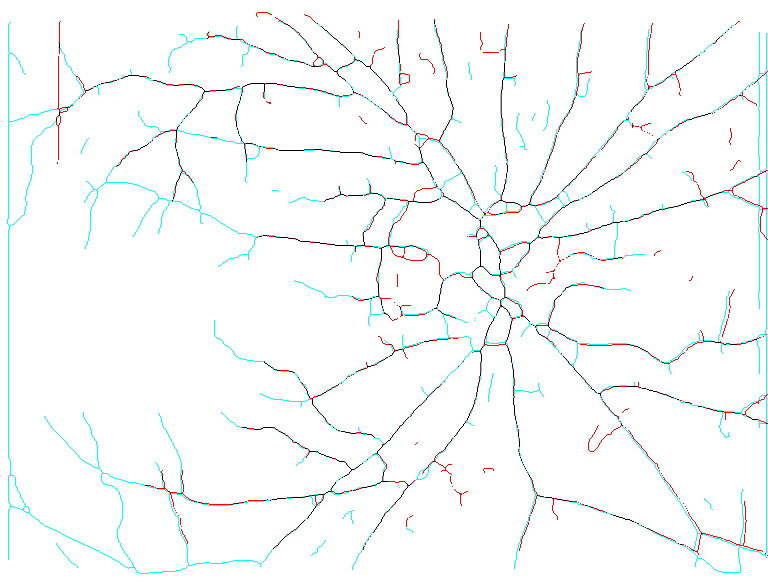
\includegraphics[width=0.3\linewidth]{128-225-initial-reg.png}}
\hspace{0.1in}
\subfigure[原始图像配准结果]{
  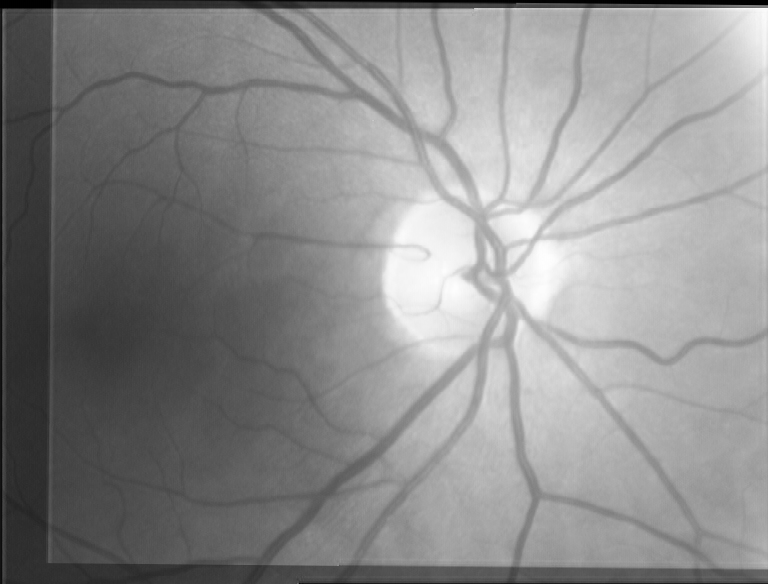
\includegraphics[width=0.3\linewidth]{128-225-initial-result.png}}
  \caption{局部初始配准}
 \end{figure}
\end{frame}


 \begin{frame}
 \frametitle{局部初始配准-分支未对齐}
  {\color{red}{当前存在问题}}:离环结构较远的区域,尤其是图像的边缘部分,经常会出现分支血管未对齐的情况。
     \begin{figure}[ht!]
    \centering
  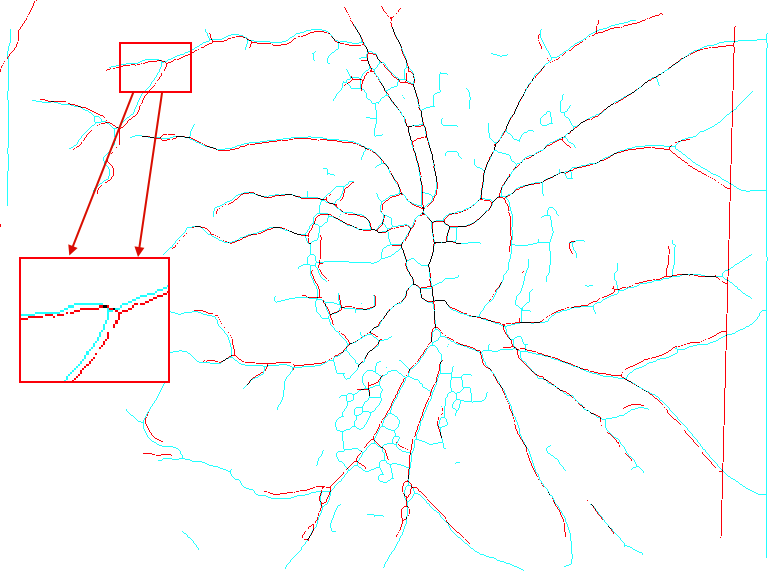
\includegraphics[width=0.6\linewidth]{067-119-initial_reg.png}
  \caption{血管未对齐的局部初始配准结果}
 \end{figure}
\end{frame}

 \begin{frame}
 \frametitle{全局二次配准}
 {\color{blue}{解决方法}}:
 \begin{itemize}
 \item 对比参考图像和待配准图像的变换后图像,找到未对齐的血管分叉点(或交叉点)。
 \item 构成环 -血管 -分叉点特征点集合,再次进行相似性变换。
 \end{itemize}
\end{frame}

 \begin{frame}
 \frametitle{全局二次配准}
  \begin{figure}[ht!]
    \centering
  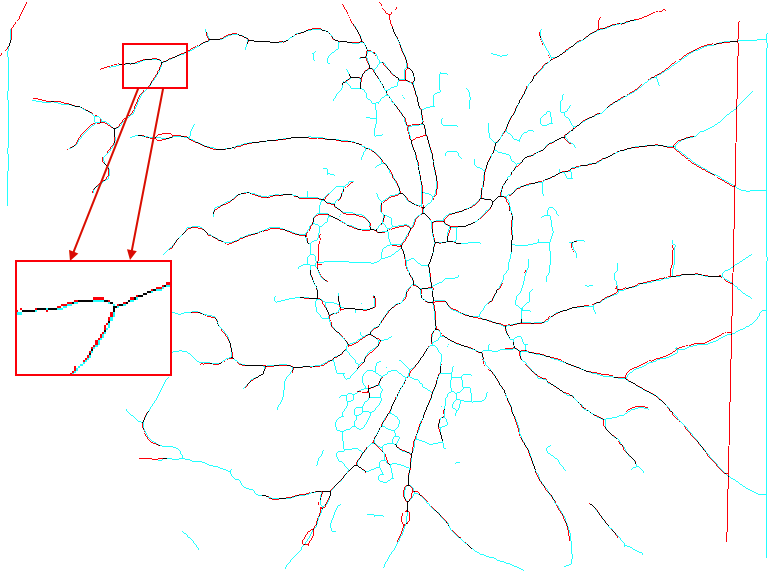
\includegraphics[width=0.6\linewidth]{067-119-glocal_reg.png}
  \caption{改善后的全局二次配准结果}
 \end{figure}
\end{frame}

\section{实验对比及分析}
\subsection{评价方法}

\begin{frame}
\frametitle{配准误差度量方法}
目前最主要的评估方法:
\begin{itemize}
\item {\color{blue}{专家主观评估}}:医务工作者或研究人员的经验判断,配准结果等级可分为4类:{\color{blue}{好(Good)}},{\color{blue}{可接受(Accepted)}},{\color{blue}{不可接受(Not Accepted)}},{\color{blue}{差(Bad)}}。

{\color{red}{效率较低,存在较多的主观因素}}。
\item {\color{blue}{客观评估}}:匹配误差、对齐误差等。
\end{itemize}
我们的方法:
\begin{itemize}
\item 成功率(Success Rate)。
\item 骨架对齐误差度量(Skeleton Alignment Error Measure),该值越小说明误差越小。
\end{itemize}
\end{frame}

\begin{frame}
\frametitle{骨架对齐误差度量}
{\color{blue}{预置条件}}:参考图像$M_i(i=1,2,\cdots,14)$,待配准图像$N_j(j=1,2,\cdots,14)$,待配准图像变换后的图像为$N_{jM_i}$。

{\color{blue}{算法步骤}}:
\begin{enumerate}
\item 对$N_{jM_i}$的每个血管点,取$7\times7$的区域,计算在参考图像对应区域内与该血管点距离最近的$M_i$上的点的欧式距离$d$。
\item 计算完成$N_j$的所有点,得SAEM定义如下:
\begin{align}
SAEM_{ijk}=\frac{(\sum d)}{Num_v}
\end{align}	 	
其中$Num_v$是$N_{jM_i}$的有效像素数。
\item 约束条件为$\frac{Num_v}{Num_{N_j}}$,并且$\frac{Num_{N_jM_i}}{Num_{N_j}}\geq 38\%$ ,其中$Num_{(.)}$代表$(.)$中的像素数量。
\end{enumerate}
\end{frame}

\begin{frame}
\frametitle{数据集}
VARIA数据库\footnote{Ortega M, Penedo M G, Rouco J, et al. Retinal verification using a feature points-based bio- metric pattern. Eurasip Journal on Advances in Signal Processing, 2009, 2009(1):1–13.}\footnote{Ortega M, Penedo M G, Rouco J, et al. Personal verification based on extraction and character- isation of retinal feature points. Journal of Visual Languages and Computing, 2009, 20(2):80– 90.},包含来自于 139 个采集者的233 幅视网膜图像,每个个体有不同数量的采集图像,因此共155对视网膜图像用于进行配准。
\end{frame}

\subsection{对比实验}

\begin{frame}
\frametitle{\ding{172}~变换模型对比}
只采用环结构特征进行配准,选择{\color{blue}{相似性变换,仿射变换和二阶多项式变换}}作为变换模型进行对比。
\begin{table}[!h]
\caption{不同变换模型的对比结果}
\centering
\begin{tabular}{lcc}
\toprule
变换模型 & 成功率(SR)& SAEM (单位:像素)\\
\midrule
相似性变换 & ${\color{blue}{95.5\%}}$ & ${\color{blue}{0.9206}}$ \\
仿射变换 & $35.48\%$ & $0.844$              \\
多项式变换& $15.48\%$ & $0.139$\\
\bottomrule
\end{tabular}
\label{models}
\end{table}
\setlength{\fboxsep}{2pt}%
     \doublebox{%
       \begin{minipage}{11cm}
实验结果证明相似性变换为最适合环结构特征的变换模型。
       \end{minipage}}
\end{frame}

\begin{frame}
\begin{figure}
\setcounter{subfigure}{0}
    \subfigure[仿射变换配准结果]{
  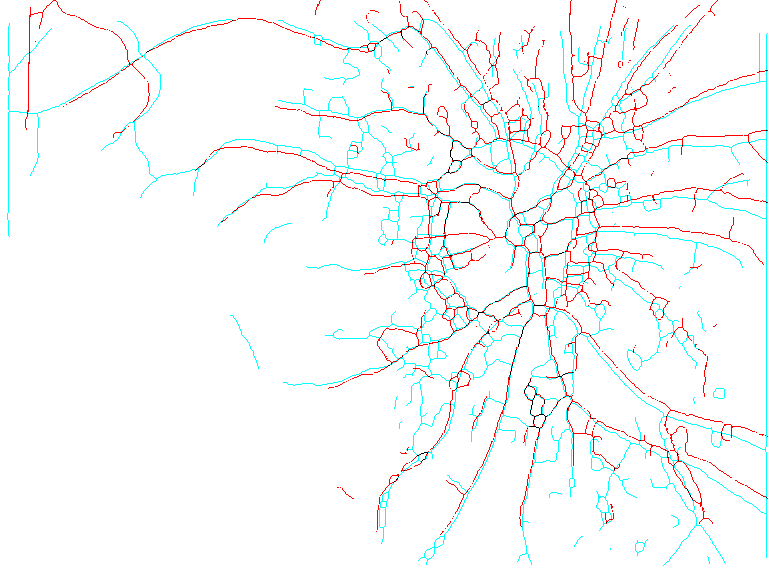
\includegraphics[width=0.35\linewidth]{R132-R133-4-3-affine-three_five-1.7024.png}}
\hspace{0.2in}
\subfigure[多项式变换配准结果]{
  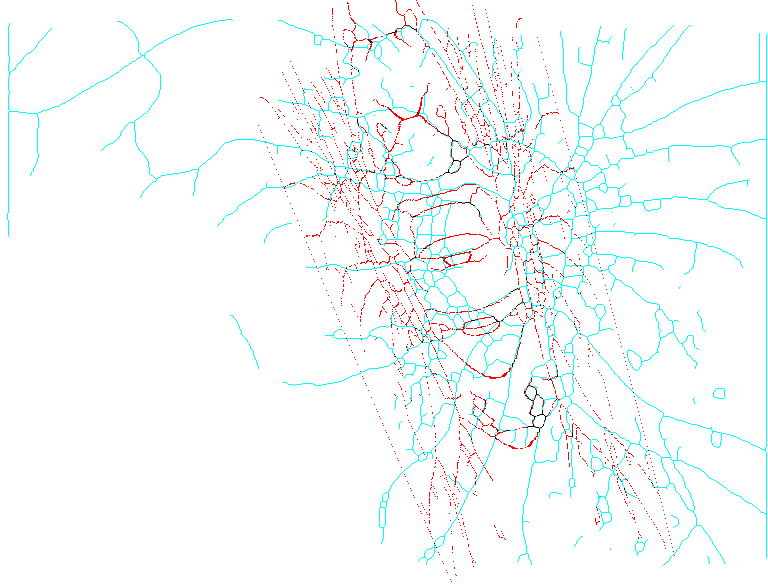
\includegraphics[width=0.35\linewidth]{R132-R133-4-3-polynomial-three_five-13.png}}
  \\
  \subfigure[相似性变换配准结果]{
  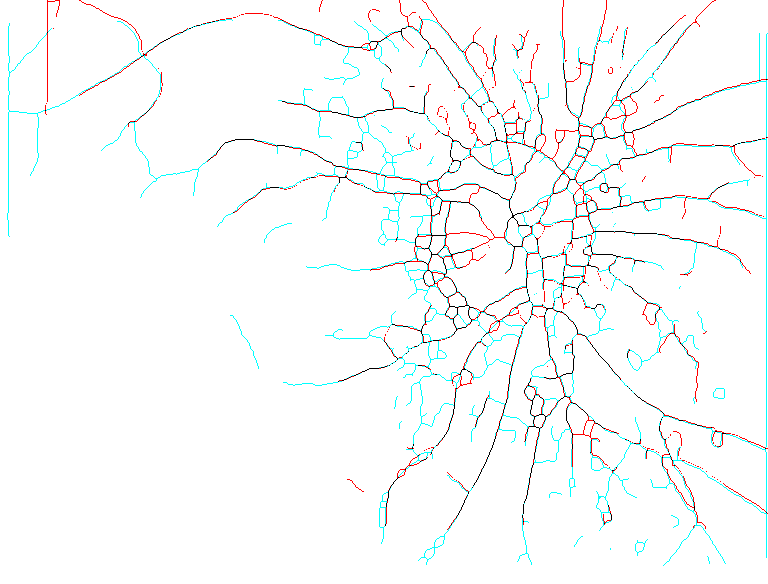
\includegraphics[width=0.35\linewidth]{R132-R133-4-3-similarity-three_five-0.84855.png}}
 \caption{不同变换模型配准结果}
\end{figure}
\end{frame}

\begin{frame}
\frametitle{\ding{173}~特征对比}
{\color{blue}{环}},{\color{blue}{环 -血管}},{\color{blue}{环 -血管 -分叉点特征}},均使用多尺度分割方法,相似性变换作为变换模型。
\begin{table}[!ht]
\caption{不同特征的对比试验结果}
\centering
\begin{tabular}{lcc}
\toprule
特征 & 成功率(SR)& SAEM (单位:像素)\\
\midrule
环特征 & $95.5\%$ & $0.921$ \\
环-血管特征 & $96.77\%$ & $0.895$              \\
环-血管-分叉点特征& ${\color{blue}{100\%}}$ & ${\color{blue}{0.873}}$\\
\bottomrule
\end{tabular}
\end{table}
\setlength{\fboxsep}{2pt}%
\doublebox{%
\begin{minipage}{11cm}
实验结果证明环 -血管 -分叉点特征是其中 最具鲁棒性的特征。
 \end{minipage}}
\end{frame}

\begin{frame}
\begin{figure}
\setcounter{subfigure}{0}
    \subfigure[环特征配准结果]{
  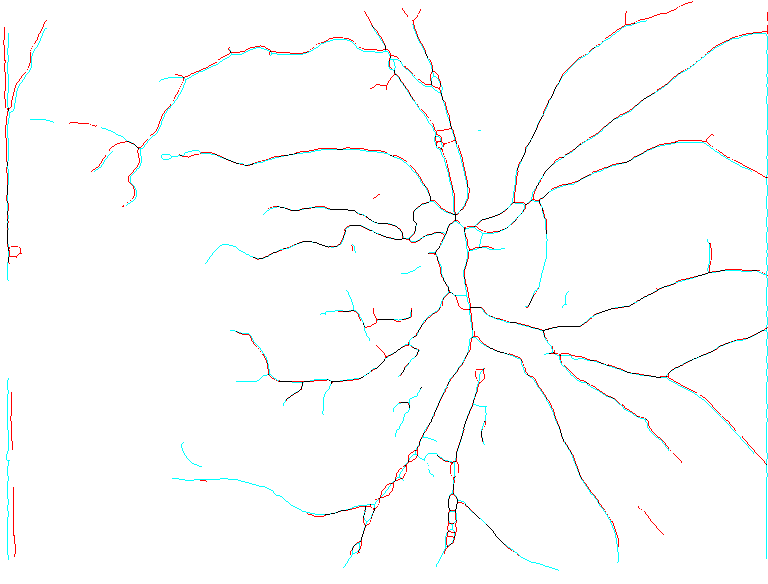
\includegraphics[width=0.35\linewidth]{R118-R119-8-9-cycle-four_five-0.90055.png}}
\hspace{0.2in}
\subfigure[环-血管特征配准结果]{
  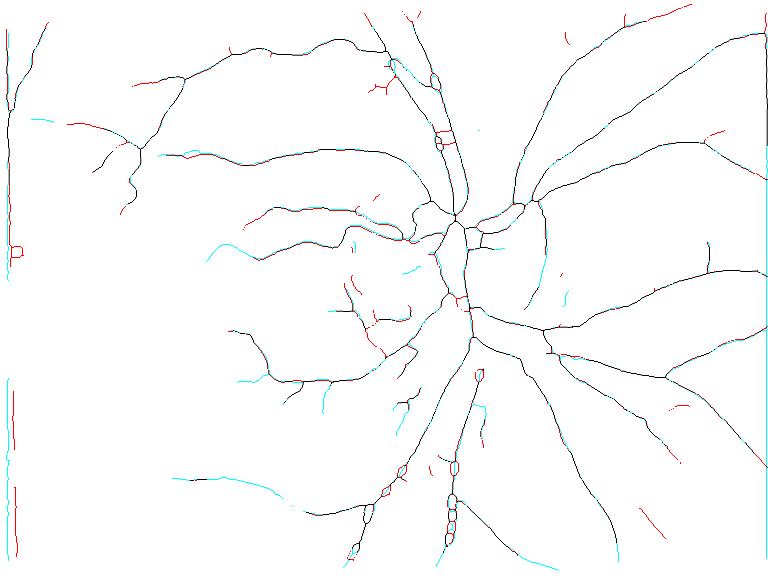
\includegraphics[width=0.35\linewidth]{R118-R119-10-6-vessel-three_four-0.64047.png}}
  \\
  \subfigure[环-血管-分叉点特征配准结果]{
  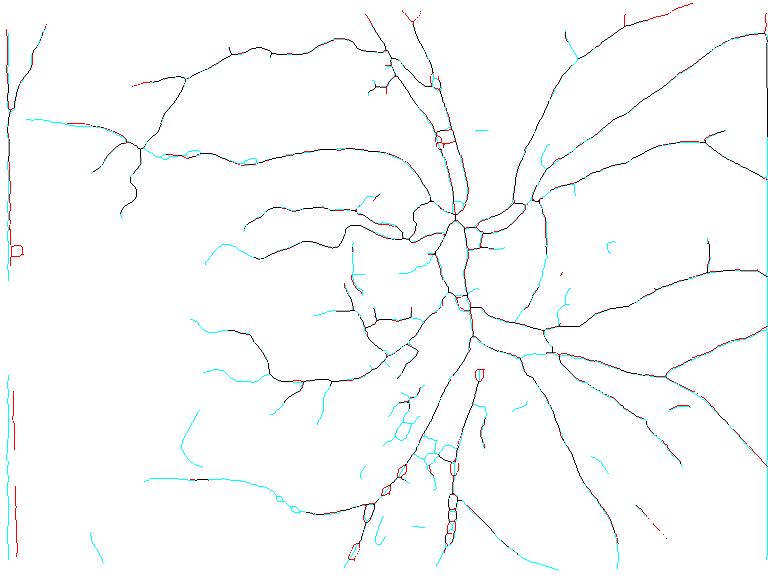
\includegraphics[width=0.3\linewidth]{R118-R119-2-6-twice-14-three_four-0.5855.png}}
 \caption{不同特征配准结果}
\end{figure}
\end{frame}

\begin{frame}
\frametitle{\ding{174}~算法对比}
与经典的结构特征方法-{\color{blue}{Bifurcation结构}}方法进行对比。

Bifurcation结构由一个主分叉点和它的三个邻域分叉点组成。
   \begin{figure}[ht!]
   \centering
  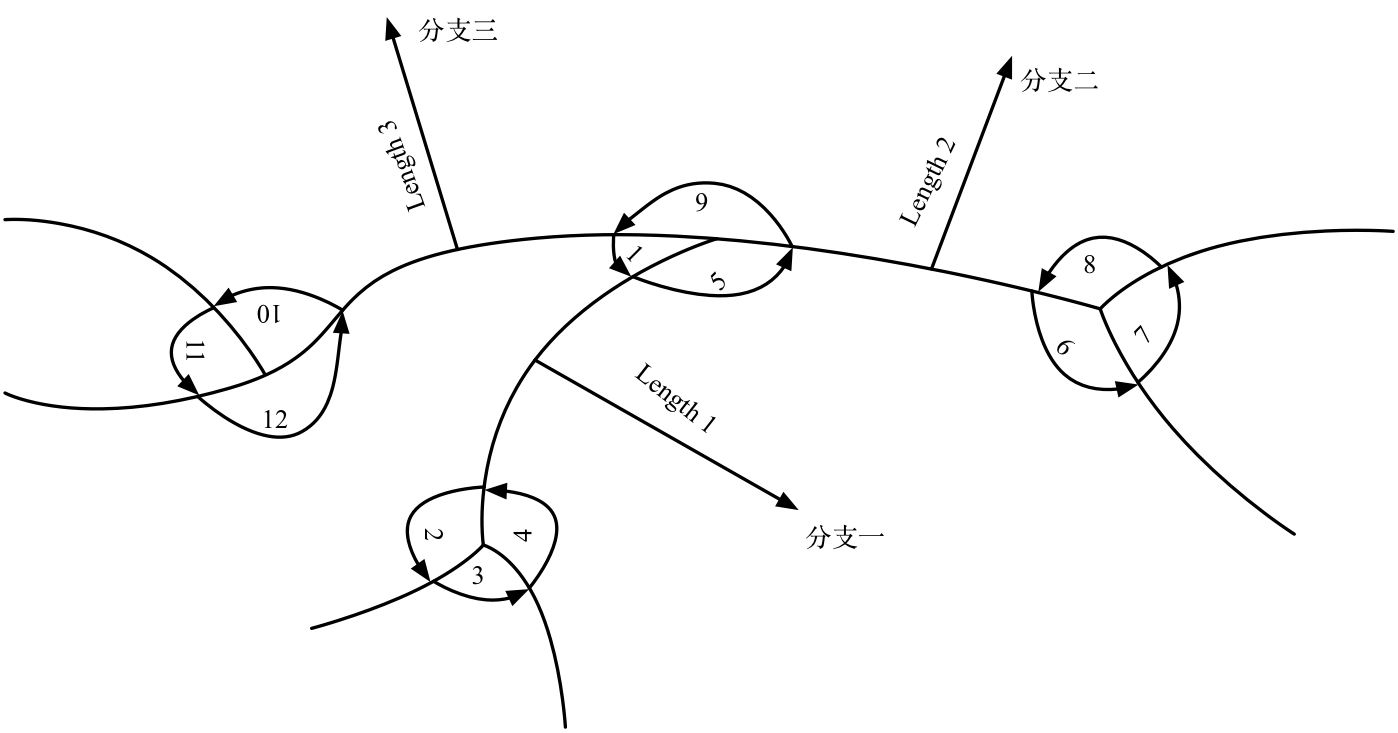
\includegraphics[width=0.7\linewidth]{bifurcate.png}
  \caption{Bifurcation结构示意图}
    \label{bifurcation}
 \end{figure}
\end{frame}

\begin{frame}
\frametitle{\ding{174}~算法对比}
\begin{table}[!ht]
\caption{不同算法的对比实验结果}
\centering
\begin{tabular}{lcc}
\toprule
方法 & 成功率(SR)& SAEM (单位:像素)\\
\midrule
Bifurcation 结构(多尺度)& $95.5\%$ & $0.937$ \\
Bifurcation 结构+Global & $96.77\%$ & $0.877$ \\
我们的方法& ${\color{blue}{100\%}}$ & ${\color{blue}{0.873}}$\\
\bottomrule
\end{tabular}
\end{table}
实验结果表明:
\begin{itemize}
\item 我们提出的环结构特征比 Bifurcation 结构更加稳定,更具有鲁棒性。
\item 我们提出的多尺度与 从局部到全局的配准策略,具有较好的通用性。
\end{itemize}
\end{frame}


\begin{frame}
\begin{figure}
\setcounter{subfigure}{0}
    \subfigure[ Bifurcation方法配准结果]{
  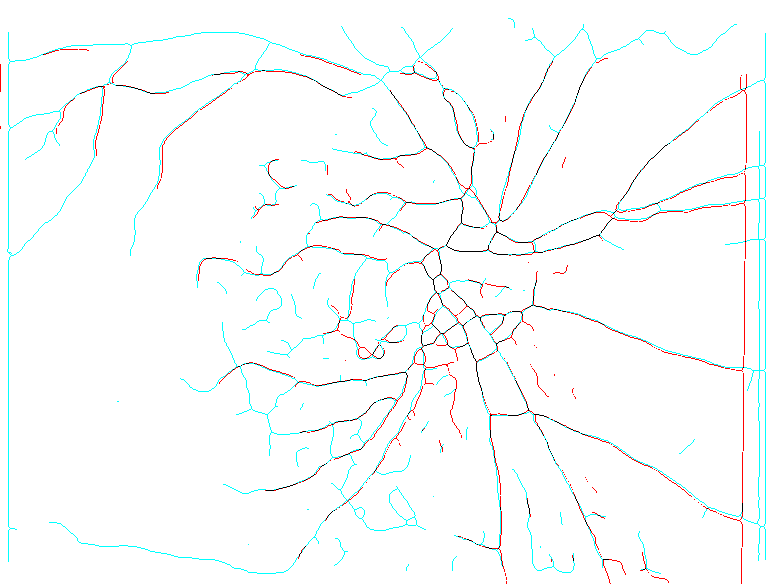
\includegraphics[width=0.35\linewidth]{R122R123-Bifurcation-Skeleton-Registration-1.0068.png}}
\hspace{0.2in}
\subfigure[BifurcationGlobal方法配准结果]{
  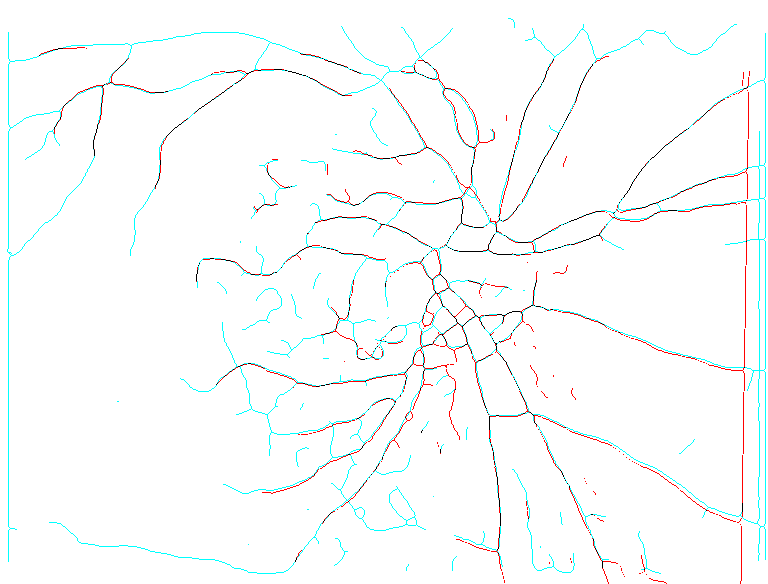
\includegraphics[width=0.35\linewidth]{R122R123-BifurcationGlobal-Skeleton-Registration-0.96393.png}}
  \\
  \subfigure[LGMM方法配准结果]{
  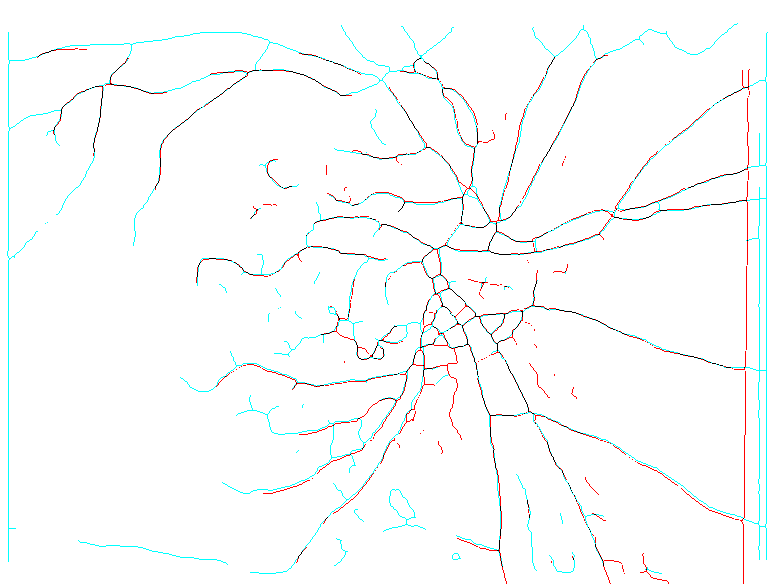
\includegraphics[width=0.3\linewidth]{R122R123-LGMM-Skeleton-Registration-twice-14-five-0.87972.png}}
 \caption{不同方法配准结果}
\end{figure}
\end{frame}

\section{总结与展望}
\begin{frame}
\frametitle{总结}
主要工作如下:
\begin{itemize}
\item 提出了一种新的视网膜配准结构特征:环结构。同时,提出了基于空间信息的深度优先搜索算法(SDFS)来提取环结构,该算法可广泛应用于无向无权图的最小环基的搜索,实现多点环结构的提取。
\item 提出了从局部到全局的配准策略。
\item 提出了配准结果度量方法:骨架化误差度量算法(SAEM),成功应用于对配准结果的评价和度量。
\end{itemize}
\end{frame}

\begin{frame}
\frametitle{展望}
在未来需要进行的一些工作:
\begin{itemize}
\item 降低整体算法复杂度。
\item 采用图片较多、更高分辨率的数据集进行实验。
\end{itemize}
\end{frame}

\begin{frame}
\vspace{2cm}

\centering{\shado{\textit{谢谢!}}}
%\centering{\color{blue} \kaishu \Huge{ \emph{\textbf{  谢谢!}}}}\\
\vspace{1.5cm}

\begin{flushright}
\emph{\href{mailto:qxx1990421@163.com}{\textrm {Xinxin~Qiu}}}\\
\href{http://www.ouc.edu.cn}{\textrm {Ocean University of China}}\\
\emph{\textrm {2016.05.22}}
\end{flushright}  
\end{frame}



\end{document}
